\documentclass[a4paper,12pt]{article}
\usepackage[left=2.5cm,right=2cm,top=3cm]{geometry}
\usepackage[utf8x]{inputenc}
\usepackage[czech]{babel}
\usepackage[IL2]{fontenc}
\usepackage{eso-pic}
\usepackage{graphicx}
\graphicspath{resources/}

\renewcommand{\baselinestretch}{1.2}

\begin{document}

	% Logo FIT
	\AddToShipoutPictureBG{
		\AtPageUpperLeft{\raisebox{-\height}{
\includegraphics[scale=0.50]{fit-logo.pdf}}}
	}
	
	% Turn off numbering
	\pagenumbering{gobble}	

	\setlength{\parindent}{0pt}
	\vspace*{10pt}
	\LARGE \textsc{Abstrakt}
	\normalsize

	\vspace*{5pt}
	\textit{Projekt do předmětu SIN - Inteligentní systémy} \\
	\textit{Téma č. 2, Subsystém inteligentní budovy} \\
	\textit{Řešitelé: Daniel Dušek (xdusek21), Anna Popková (xpopko00)}

	\setlength{\parindent}{15pt}
	\setlength{\parskip}{15pt}
	\renewcommand{\baselinestretch}{1.5}
	\vspace*{15pt}
	
	\section{Úvod}

    V projektu je navržen subsystém inteligentní budovy - konkrétně podsystém řídící prostředí v ložnici. Prostředí v ložnici je řízeno tak, aby poskytovalo ideální světelné a tepelné podmínky pro spánek a zároveň umožňovalo uživateli, popř. uživatelům ložnice nastavovat úroveň vlhkosti vzduchu. Nad tímto subsystémem je v rámci projektu prováděna simulace, která demonstruje schopnost systému reagovat na změny podmínek uvnitř i vně ložnice. 

    Projekt uvažuje, že se v ložnici nachází následující ovladatelná zařízení: topení, klimatizace, zvlhčovač a odvlhčovač vzduchu (v realitě by mohlo jít pouze o jedno zařízení), automatické rolety a chladné diodové osvětelní simulující sluneční svit. Dále se v ložnici a~mimo ni nachází dvojice tepelných senzorů, dvojice senzorů vlhkosti a jeden senzor úrovně osvětlení uvnitř ložnice.

    Inteligentní systém dohlíží na to, aby v místnosti byla neustále udržována teplota nastavená uživateli - toto realizuje střídavým zapínáním a vypínáním topení, popřípadě klimatizace. Dále systém dle uživatelsky nastavených hodnot připravuje prostředí pro pohodlné vstávání - rozsvicením diod simulujících sluneční svit v době vstávání - a také pro klidný noční spánek - zatahováním rolet a tlumením světla v době ukládání se ke spánku. Uživatel může zmíněné hodnoty nastavovat prostřednictvím nástroje Domoticz - v sekci \uv{Setup $>$ User variables}. Systém také informuje uživatele  o aktuální vlhkosti ve vzduchu a umožňuje zapnout zvlhčování či odvlhčování místnosti. Zapínání a vypínání zvlhčování vzduchu uživatel realizuje opět skrze Domoticz rozhraní a to zapnutím či vypnutím přepínačů \uv{Humidifier} a \uv{Dehumidifier}. Stejným způsobem lze vytáhnout či zatáhnout automatické rolety a vypnout či zapnout umělé osvětlení v časech, kdy je od nich očekáváno konkrétní nastavení. V reálném světě by tyto přepínače a indikátory umístěné v Domoticz online rozhraní byly pravděpodobně realizovány formou hardwarového ovládacího panelu u dveří do místnosti, v~konkrétním případě inteligentní ložnice pak možná v blízkosti postele.

    Demonstrace funkčnosti subsystému implementovaného v tomto projektu využívá simulace konkrétních dnů v roce. Poměr reálný čas ku simulačnímu času je zvolen tak, že jedna sekunda reálného času odpovídá 10 minutám simulačního času. Během startu simulace je vybrán náhodný den v roce, od kterého začne simulace probíhat. Od náhodně zvoleného dne v roce se odvíjí hodnoty teploty, vlhkosti a slunečního svitu naměřené na senzorech umístěných v místnosti a mimo ni. Změna venkovních podmínek se promítá změnou hodnot na~senzorech a inteligentní subsystém na tyto změny reaguje.


    \section{Příprava prostředí a spuštění simulace}

    Pro implementaci a simulaci inteligentního subsystému bylo využito knihovny JADE pro~jednoduchou implementaci agentního prostředí v jazyce JAVA. Pro řízení a zobrazování stavů zařízení v prostředí je využíváno nástroje Domoticz. V této sekci jsou popsány kroky, které je nutné učinit pro úspěšné spuštění projektu. 

    \subsection{Příprava Domoticz prostředí}
    Projekt využívá pro zobrazování aktuálních hodnot nástroj Domoticz, který je nutné mít nainstalovaný na počítači, spuštěný na portu \textbf{8888} (defaultně je instalován na port 8080). Implementovaný projekt předpokládá, že zastihne Domoticz na adrese \textit{http://127.0.0.1:8888}. Není-li možné spustit Domoticz na požadované adrese, je třeba upravit hodnotu vlastnosti třídy \textit{SmartBedroomAgent} \textbf{domoticzBaseUrl} tak, aby ukazovala na reálnou adresu na které je nástroj spuštěn. Spouštíte-li projekt z přibaleného *.jar souboru, je nutné, aby Domoticz běžel na právě zmíněné adrese.

    Během inicializační fáze při spouštění projektu jsou vytvořeny všechny uživatelské proměnné, zařízení a HW v Domoticz databázi prostřednictvím REST API, které poskytuje. Je však nutné navigovat v Domoticzu do \uv{Setup $>$ Events} a přidat LUA skript reagující na~změnu zařízení (možnost \uv{\textit{Device}}), pojmenovaný \uv{\textit{HeaterControl}} a označený jako aktivní. Obsah tohoto skriptu je možné nalézt v přiloženém souboru k projektu \textit{DomoticzHeaterControl.lua}.

    Po splnění těchto podmínek začne subsystém řídit a fungovat. Pod záložkami \uv{\textit{Temperature}}, \uv{\textit{Light}} a \uv{\textit{Switch}} je možné sledovat stav zařízení a popřípadě jej měnit. 

    \subsection{Spuštění projektu prostřednictvím INSTALL a RUN skriptů}
    S projektem jsou odevzdávány skripty INSTALL a RUN ve verzích pro Windows (přípona .ps1, spustitelné ve Windows PowerShell) a Linux (přípona .sh). Spuštěním INSTALL skriptu dojde ke stažení *.jar souboru z autorova školního účtu na adrese \textit{stud.fit.vutbr.cz}. Následné spuštění skriptu RUN spustí tento stažený *.jar soubor a simulace započne. Stejně jako výše platí, že tento *.jar soubor očekává běžící instanci Domoticz nástroje na lokální \texttt{127.0.0.1} adrese na portu \texttt{8888}.

    \subsection{Spouštění projektu ze zdrojového kódu}
    Ve složce \uv{\textit{Sources}} je přibalená kompletní adresářová struktura rozložením odpovídající struktuře \textit{Maven} projektu. Při otevření ve vhodném JAVA IDE (například \textit{IntelliJ}) je třeba nastavit tzv. \textit{Run Configuration} tak, že \textit{Main} třída je \textit{jade.Boot} a parametr spuštění je nastaven na \textit{-gui "WorldAgent:Agents.WorldAgent;"}. Potom je třeba spustit Maven re-import proces, a spuštění vytvořené konfigurace úspěšně přeloží a~nastartujte projekt.

    \section{Implementace}

    Implementovaná aplikace odděluje logiku řízení od samotného řízení a to tak, že logika řízení je realizována na straně nástroje Domoticz, řízení dle rozhodnutí učiněných v nástroji Domoticz je realizováno na straně JAVA aplikace.
    
    V aplikaci vystupují dva dominantní agenti \textit{WorldAgent} a \textit{SmartBedroomAgent}. \textit{WorldAgent} je simulační agent představující vnější svět a také zdroj dat pro senzory. \textit{SmartBedroomAgent} zastává roli styčného důstojníka mezi logickou částí řízení, senzory a aktivními zařízeními v subsystému. \textit{SmartBedroomAgent} na základě rozhodnutí provedených nástrojem Domoticz předává řídící příkazy zařízením uvnitř ložnice, které má ve své správě. 

    Každé z aktivních zařízení v ložnici je taktéž realizováno jako agent. Tito agenti pak informují na základě svých stavů (aktivní či neaktivní) svět o tom, že běží. Svět (a tedy \textit{WorldAgent}) na základě této informace pak upravuje hodnoty reprezentující teplotu, vlhkost a osvětlení v místnosti v reálném světě.

    \textit{SmartBedroomAgent} je také zodpovědný za získávání dat od reálného světa a odpovídajícího nastavování svých senzorů. Informace ze senzorů pak pravidelně sděluje Domoticz nástroji.

    \subsection{Agenti}
    \textbf{WorldAgent} - Simuluje změny v okolním světě. Je zodpovědný za změny teploty v průběhu dne a v průběhu roku. Informace pro tyto změny čerpá z průměrných teplot v ČR v průběhu roku a náhodně osciluje v jejich blízkosti. Dále je zodpovědný za změnu vlhkosti vzduchu a jasu světla v průběhu dne. Informace jsou opět čerpány na základně průměrných hodnot v ČR v průběhu roku. Přijme-li WorldAgent informaci od některého z aktivních zařízení, že pracuje, promítne odpovídající změny do aktuálního stavu světa (příklad: topení (\textit{Heater} zašle zprávu, že se aktivoval, WorldAgent na základě této informace zvedne s korekcí vůči teplotě venku, teplotu uvnitř místnosti)).
    
    \textbf{SmartBedroomAgent} - Komunikuje s \textit{WorldAgent} a žádá ho o pravidelné zprávy o změnách podmínek v reálném světě. Data z těchto podmínek zpracovává a nastavuje svým vnitřním vlastnostem, které slouží jako senzory. Informace z těchto senzorů následně komunikuje směrem k nástroji Domoticz. Přijímá řídící příkazy od Domoticz nástroje, které říkají jaké zařízení by se mělo aktivovat nebo deaktivovat. Tyto řídící příkazy deleguje prostřednictvím zpráv aktivním zařízením v místnosti. 
    
    \textbf{Humidifier, Dehumidifier} - Tito agenti zvyšují respektive snižují úroveň vlhkosti v místnosti. Reagují na zprávu od \textit{SmartBedroomAgent}, na základě které se aktivují nebo deaktivují. V pravidelných intervalech posílají zprávu \textit{WorldAgent} o tom, že jsou aktivní. \textit{WorldAgent} na základě těchto zpráv upravuje podmínky v simulačním světě.
    
    \textbf{Heater, Cooler} - Agenti zodpovědní za zvyšování respektive snižování teploty v místnosti. (De)aktivováni zprávou od \textit{SmartBedroomAgent}, jsou-li aktivní, pravidelně o této skutečnosti informují \textit{WorldAgent}.
    
    \textbf{Illuminator, Dimmer} - Agenti reprenzetující osvětlující diody a rolety. (De)aktivováni jsou na základě zprávy od \textit{SmartBedroomAgent}, který obdrží od Domaticz nástroje informaci o tom, že je je třeba aktivovat na základě uživatelsky předvolených proměnných (tedy nastavení kdy chce uživatel spát a vstávat).

    \subsection{Hierarchie agentů}
    Na nejvyšší úrovni v systému vystupují agenti \textit{WorldAgent} a \textit{SmartBedroomAgent}, kde druhý jmenovaný přijímá řídící příkazy od nástroje Domoticz, který je také možné považovat za agenta v tomto systému. Byl-li by uvažován za agenta v tomto systému, pak by byl ještě o úroveň výše než \textit{WorldAgent} a \textit{SmartBedroomAgent}. Pod \textit{SmartBedroomAgent} jsou umístěny agenti reprezentující aktivní zařízení v místnosti. Tyto aktivní zařízení přijímají příkazy od \textit{BedroomAgent} a v případě, že jsou na vyžádání aktivní, hlásí tuto informaci \textit{WorldAgent}, který ji dle svých pravidel zpracovává a promítá do aktuálního stavu světa. Hierarchie je k náhlédnutí na obrázku 1.

    \begin{figure}[h!]
        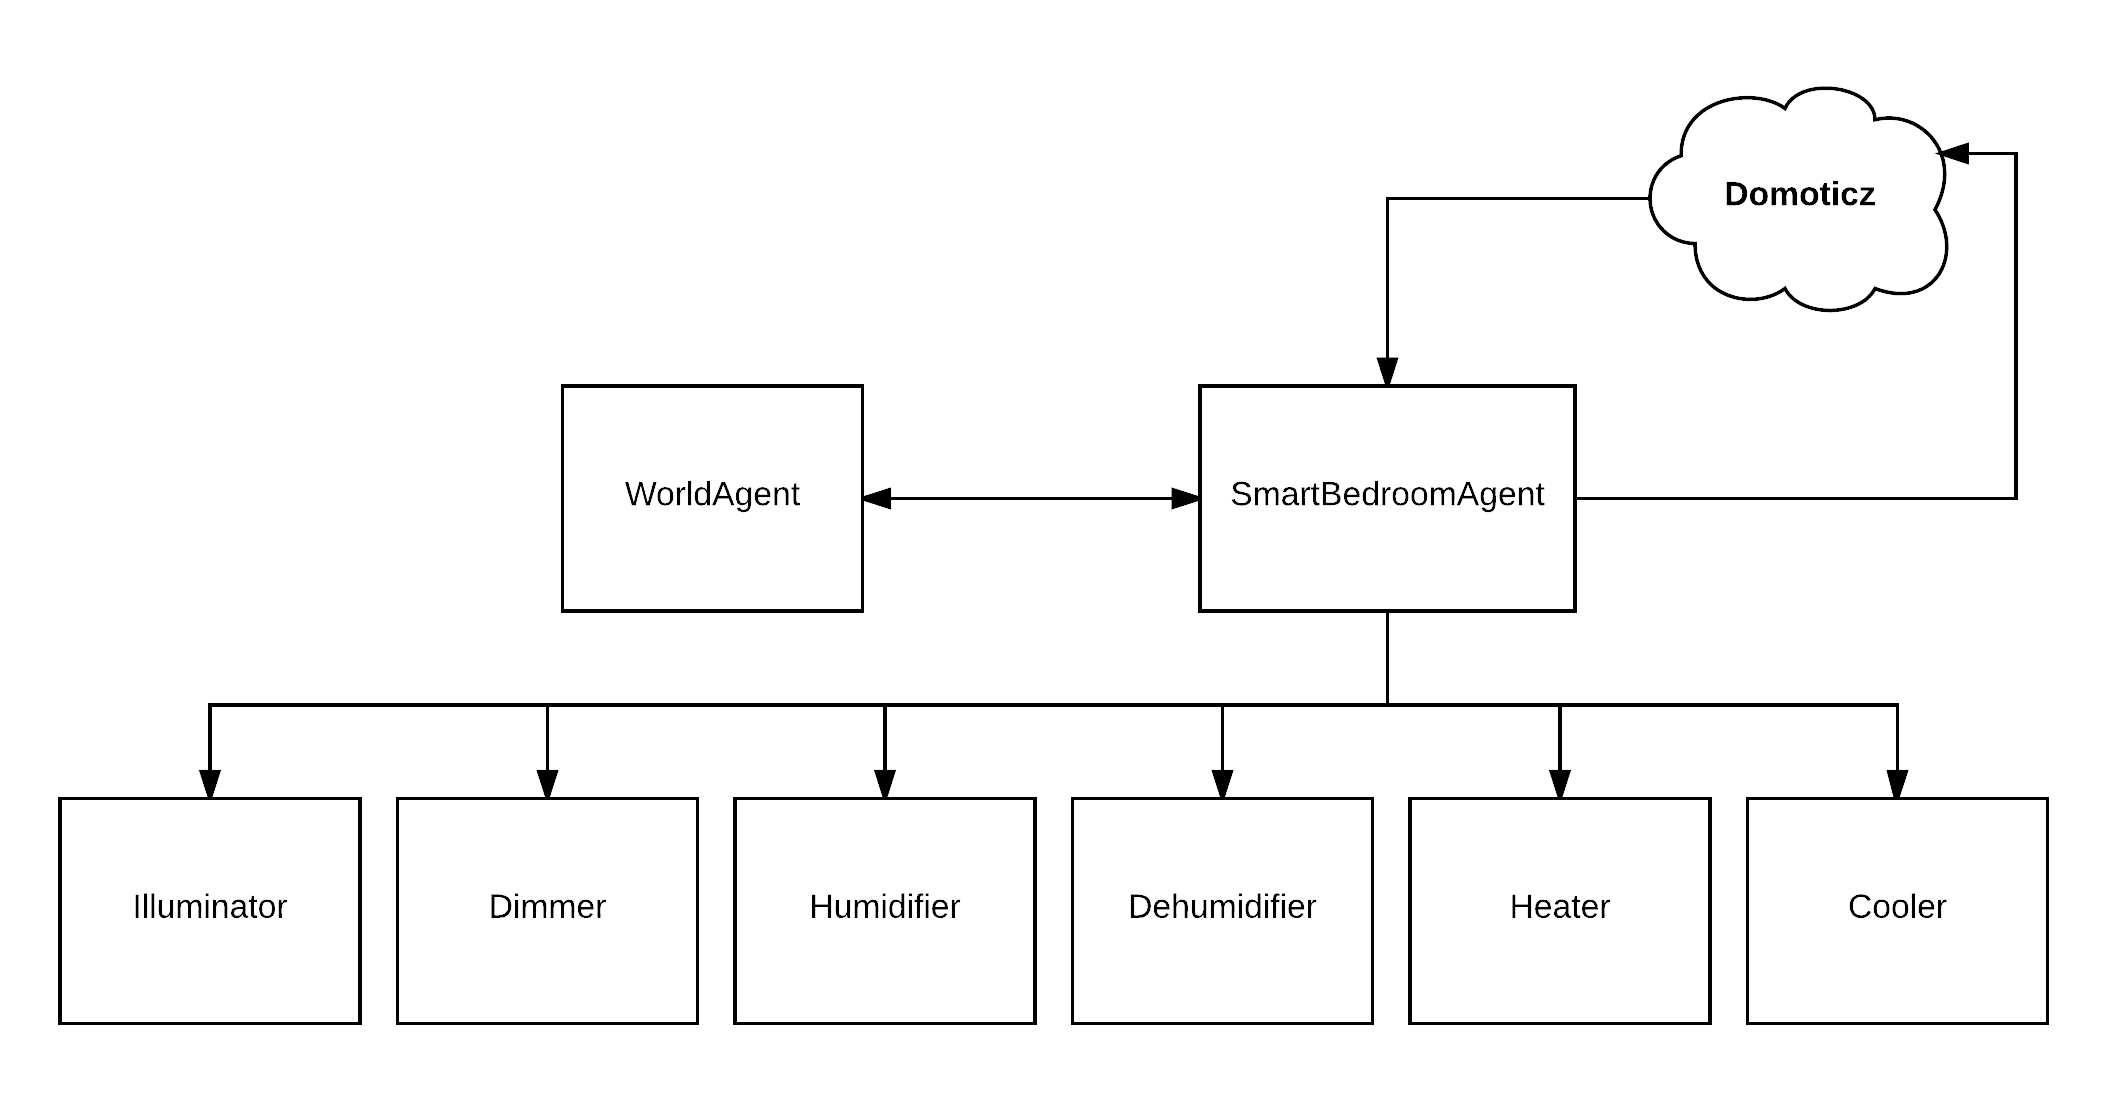
\includegraphics[scale=0.22]{resources/AgentHierarchy.png}
        \caption{Hierarchie agentů}
    \end{figure}

    % \subsection{Komunikace s nástrojem Domoticz}
    % TBD... yeah, sure.

	
\end{document}